% Created by tikzDevice version 0.12.3.1 on 2022-09-01 15:52:07
% !TEX encoding = UTF-8 Unicode
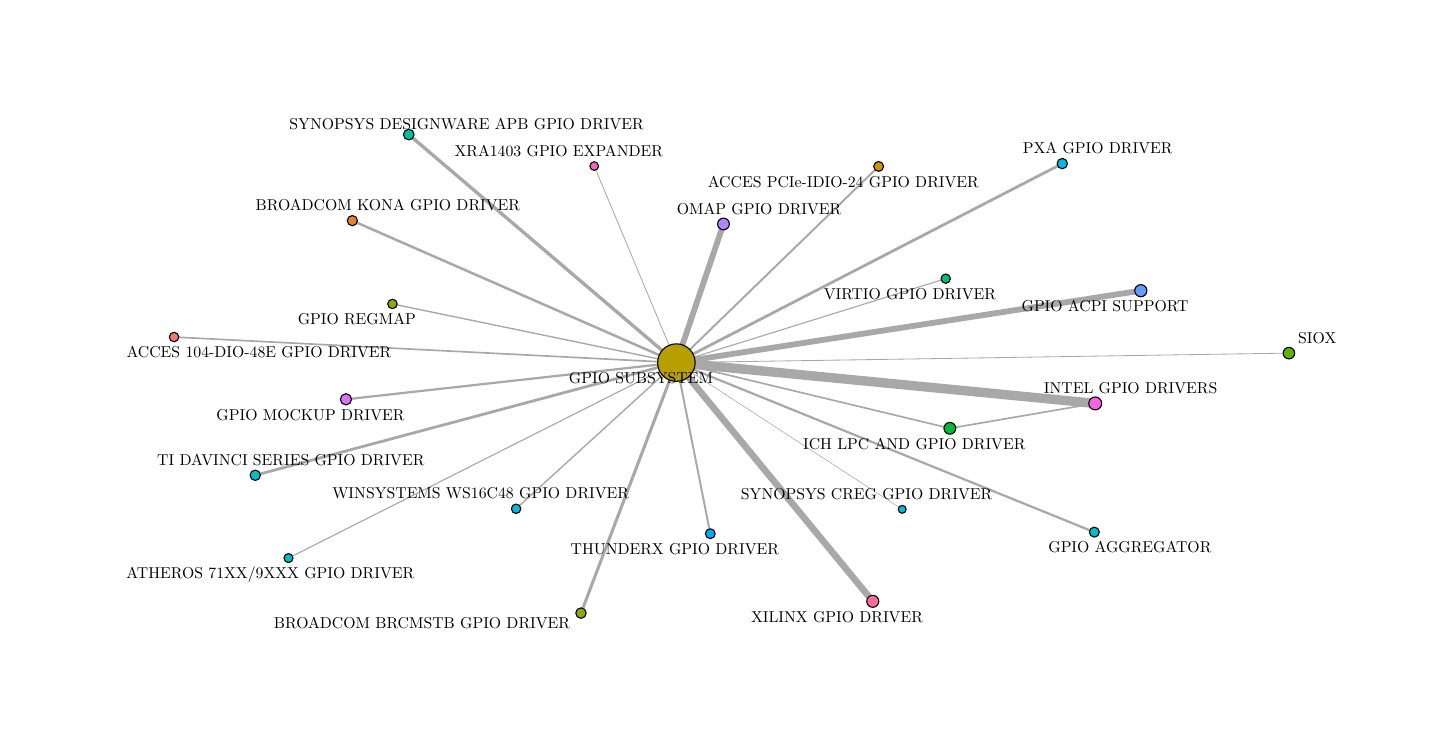
\begin{tikzpicture}[x=1pt,y=1pt]
\definecolor{fillColor}{RGB}{255,255,255}
\path[use as bounding box,fill=fillColor,fill opacity=0.00] (0,0) rectangle (505.89,252.94);
\begin{scope}
\path[clip] (  0.00,  0.00) rectangle (505.89,252.94);
\definecolor{fillColor}{RGB}{255,255,255}

\path[fill=fillColor] (  0.00,  0.00) rectangle (505.89,252.94);
\end{scope}
\begin{scope}
\path[clip] ( 32.75, 32.75) rectangle (475.89,222.94);
\definecolor{drawColor}{gray}{0.66}

\path[draw=drawColor,line width= 0.6pt,line join=round] ( 52.89,141.15) -- (234.41,131.91);

\path[draw=drawColor,line width= 0.7pt,line join=round] (307.49,202.80) -- (234.41,131.91);

\path[draw=drawColor,line width= 0.4pt,line join=round] ( 94.25, 61.27) -- (234.41,131.91);

\path[draw=drawColor,line width= 1.1pt,line join=round] (199.94, 41.40) -- (234.41,131.91);

\path[draw=drawColor,line width= 0.9pt,line join=round] (117.32,183.20) -- (234.41,131.91);

\path[draw=drawColor,line width= 2.1pt,line join=round] (402.23,157.89) -- (234.41,131.91);

\path[draw=drawColor,line width= 0.8pt,line join=round] (385.44, 70.65) -- (234.41,131.91);

\path[draw=drawColor,line width= 0.8pt,line join=round] (115.01,118.64) -- (234.41,131.91);

\path[draw=drawColor,line width= 0.5pt,line join=round] (131.81,153.11) -- (234.41,131.91);

\path[draw=drawColor,line width= 0.6pt,line join=round] (234.41,131.91) -- (333.23,108.17);

\path[draw=drawColor,line width= 3.4pt,line join=round] (234.41,131.91) -- (385.75,117.16);

\path[draw=drawColor,line width= 2.1pt,line join=round] (234.41,131.91) -- (251.43,182.00);

\path[draw=drawColor,line width= 1.0pt,line join=round] (234.41,131.91) -- (373.85,203.82);

\path[draw=drawColor,line width= 0.3pt,line join=round] (234.41,131.91) -- (455.75,135.34);

\path[draw=drawColor,line width= 0.2pt,line join=round] (234.41,131.91) -- (316.01, 78.90);

\path[draw=drawColor,line width= 1.2pt,line join=round] (234.41,131.91) -- (137.71,214.30);

\path[draw=drawColor,line width= 0.7pt,line join=round] (234.41,131.91) -- (246.66, 70.09);

\path[draw=drawColor,line width= 1.0pt,line join=round] (234.41,131.91) -- ( 82.23, 91.20);

\path[draw=drawColor,line width= 0.4pt,line join=round] (234.41,131.91) -- (331.73,162.24);

\path[draw=drawColor,line width= 0.5pt,line join=round] (234.41,131.91) -- (176.49, 79.10);

\path[draw=drawColor,line width= 2.4pt,line join=round] (234.41,131.91) -- (305.37, 45.65);

\path[draw=drawColor,line width= 0.3pt,line join=round] (234.41,131.91) -- (204.72,202.93);

\path[draw=drawColor,line width= 0.6pt,line join=round] (333.23,108.17) -- (385.75,117.16);
\definecolor{drawColor}{RGB}{0,0,0}
\definecolor{fillColor}{RGB}{248,118,109}

\path[draw=drawColor,line width= 0.4pt,line join=round,line cap=round,fill=fillColor] ( 52.89,141.15) circle (  1.71);
\definecolor{fillColor}{RGB}{211,146,0}

\path[draw=drawColor,line width= 0.4pt,line join=round,line cap=round,fill=fillColor] (307.49,202.80) circle (  1.78);
\definecolor{fillColor}{RGB}{0,191,196}

\path[draw=drawColor,line width= 0.4pt,line join=round,line cap=round,fill=fillColor] ( 94.25, 61.27) circle (  1.63);
\definecolor{fillColor}{RGB}{147,170,0}

\path[draw=drawColor,line width= 0.4pt,line join=round,line cap=round,fill=fillColor] (199.94, 41.40) circle (  1.89);
\definecolor{fillColor}{RGB}{232,133,38}

\path[draw=drawColor,line width= 0.4pt,line join=round,line cap=round,fill=fillColor] (117.32,183.20) circle (  1.84);
\definecolor{fillColor}{RGB}{97,156,255}

\path[draw=drawColor,line width= 0.4pt,line join=round,line cap=round,fill=fillColor] (402.23,157.89) circle (  2.19);
\definecolor{fillColor}{RGB}{0,191,196}

\path[draw=drawColor,line width= 0.4pt,line join=round,line cap=round,fill=fillColor] (385.44, 70.65) circle (  1.80);
\definecolor{fillColor}{RGB}{219,114,251}

\path[draw=drawColor,line width= 0.4pt,line join=round,line cap=round,fill=fillColor] (115.01,118.64) circle (  2.03);
\definecolor{fillColor}{RGB}{147,170,0}

\path[draw=drawColor,line width= 0.4pt,line join=round,line cap=round,fill=fillColor] (131.81,153.11) circle (  1.70);
\definecolor{fillColor}{RGB}{183,159,0}

\path[draw=drawColor,line width= 0.4pt,line join=round,line cap=round,fill=fillColor] (234.41,131.91) circle (  6.78);
\definecolor{fillColor}{RGB}{0,186,56}

\path[draw=drawColor,line width= 0.4pt,line join=round,line cap=round,fill=fillColor] (333.23,108.17) circle (  2.13);
\definecolor{fillColor}{RGB}{245,100,227}

\path[draw=drawColor,line width= 0.4pt,line join=round,line cap=round,fill=fillColor] (385.75,117.16) circle (  2.33);
\definecolor{fillColor}{RGB}{174,135,255}

\path[draw=drawColor,line width= 0.4pt,line join=round,line cap=round,fill=fillColor] (251.43,182.00) circle (  2.12);
\definecolor{fillColor}{RGB}{0,185,227}

\path[draw=drawColor,line width= 0.4pt,line join=round,line cap=round,fill=fillColor] (373.85,203.82) circle (  1.87);
\definecolor{fillColor}{RGB}{94,179,0}

\path[draw=drawColor,line width= 0.4pt,line join=round,line cap=round,fill=fillColor] (455.75,135.34) circle (  2.08);
\definecolor{fillColor}{RGB}{0,185,227}

\path[draw=drawColor,line width= 0.4pt,line join=round,line cap=round,fill=fillColor] (316.01, 78.90) circle (  1.43);
\definecolor{fillColor}{RGB}{0,193,159}

\path[draw=drawColor,line width= 0.4pt,line join=round,line cap=round,fill=fillColor] (137.71,214.30) circle (  1.93);
\definecolor{fillColor}{RGB}{0,173,250}

\path[draw=drawColor,line width= 0.4pt,line join=round,line cap=round,fill=fillColor] (246.66, 70.09) circle (  1.78);
\definecolor{fillColor}{RGB}{0,191,196}

\path[draw=drawColor,line width= 0.4pt,line join=round,line cap=round,fill=fillColor] ( 82.23, 91.20) circle (  1.88);
\definecolor{fillColor}{RGB}{0,191,116}

\path[draw=drawColor,line width= 0.4pt,line join=round,line cap=round,fill=fillColor] (331.73,162.24) circle (  1.69);
\definecolor{fillColor}{RGB}{0,185,227}

\path[draw=drawColor,line width= 0.4pt,line join=round,line cap=round,fill=fillColor] (176.49, 79.10) circle (  1.71);
\definecolor{fillColor}{RGB}{255,105,156}

\path[draw=drawColor,line width= 0.4pt,line join=round,line cap=round,fill=fillColor] (305.37, 45.65) circle (  2.17);
\definecolor{fillColor}{RGB}{255,97,195}

\path[draw=drawColor,line width= 0.4pt,line join=round,line cap=round,fill=fillColor] (204.72,202.93) circle (  1.56);

\node[text=drawColor,anchor=base,inner sep=0pt, outer sep=0pt, scale=  0.57] at ( 83.57,133.66) {ACCES 104-DIO-48E GPIO DRIVER};

\node[text=drawColor,anchor=base,inner sep=0pt, outer sep=0pt, scale=  0.57] at (294.73,195.36) {ACCES PCIe-IDIO-24 GPIO DRIVER};

\node[text=drawColor,anchor=base,inner sep=0pt, outer sep=0pt, scale=  0.57] at ( 87.68, 53.82) {ATHEROS 71XX/9XXX GPIO DRIVER};

\node[text=drawColor,anchor=base,inner sep=0pt, outer sep=0pt, scale=  0.57] at (142.48, 35.76) {BROADCOM BRCMSTB GPIO DRIVER};

\node[text=drawColor,anchor=base,inner sep=0pt, outer sep=0pt, scale=  0.57] at (130.15,186.76) {BROADCOM KONA GPIO DRIVER};

\node[text=drawColor,anchor=base,inner sep=0pt, outer sep=0pt, scale=  0.57] at (389.31,150.38) {GPIO ACPI SUPPORT};

\node[text=drawColor,anchor=base,inner sep=0pt, outer sep=0pt, scale=  0.57] at (398.28, 63.17) {GPIO AGGREGATOR};

\node[text=drawColor,anchor=base,inner sep=0pt, outer sep=0pt, scale=  0.57] at (102.21,111.16) {GPIO MOCKUP DRIVER};

\node[text=drawColor,anchor=base,inner sep=0pt, outer sep=0pt, scale=  0.57] at (118.94,145.61) {GPIO REGMAP};

\node[text=drawColor,anchor=base,inner sep=0pt, outer sep=0pt, scale=  0.57] at (221.62,124.45) {GPIO SUBSYSTEM};

\node[text=drawColor,anchor=base,inner sep=0pt, outer sep=0pt, scale=  0.57] at (320.38,100.69) {ICH LPC AND GPIO DRIVER};

\node[text=drawColor,anchor=base,inner sep=0pt, outer sep=0pt, scale=  0.57] at (398.55,120.72) {INTEL GPIO DRIVERS};

\node[text=drawColor,anchor=base,inner sep=0pt, outer sep=0pt, scale=  0.57] at (264.30,185.56) {OMAP GPIO DRIVER};

\node[text=drawColor,anchor=base,inner sep=0pt, outer sep=0pt, scale=  0.57] at (386.65,207.36) {PXA GPIO DRIVER};

\node[text=drawColor,anchor=base,inner sep=0pt, outer sep=0pt, scale=  0.57] at (466.00,138.90) {SIOX};

\node[text=drawColor,anchor=base,inner sep=0pt, outer sep=0pt, scale=  0.57] at (303.13, 82.48) {SYNOPSYS CREG GPIO DRIVER};

\node[text=drawColor,anchor=base,inner sep=0pt, outer sep=0pt, scale=  0.57] at (158.61,216.01) {SYNOPSYS DESIGNWARE APB GPIO DRIVER};

\node[text=drawColor,anchor=base,inner sep=0pt, outer sep=0pt, scale=  0.57] at (233.85, 62.62) {THUNDERX GPIO DRIVER};

\node[text=drawColor,anchor=base,inner sep=0pt, outer sep=0pt, scale=  0.57] at ( 95.09, 94.78) {TI DAVINCI SERIES GPIO DRIVER};

\node[text=drawColor,anchor=base,inner sep=0pt, outer sep=0pt, scale=  0.57] at (318.80,154.74) {VIRTIO GPIO DRIVER};

\node[text=drawColor,anchor=base,inner sep=0pt, outer sep=0pt, scale=  0.57] at (163.68, 82.66) {WINSYSTEMS WS16C48 GPIO DRIVER};

\node[text=drawColor,anchor=base,inner sep=0pt, outer sep=0pt, scale=  0.57] at (292.44, 38.13) {XILINX GPIO DRIVER};

\node[text=drawColor,anchor=base,inner sep=0pt, outer sep=0pt, scale=  0.57] at (191.92,206.47) {XRA1403 GPIO EXPANDER};
\end{scope}
\end{tikzpicture}
